%%==================================================
%% chapter01.tex for BIT Master Thesis
%% modified by yang yating
%% version: 0.1
%% last update: Dec 25th, 2016
%%==================================================
\chapter{绪论}
\label{chap:intro}
\section{研究背景}

随着互联网的迅猛发展,各种应用软件日益增多,软件规模越来越大,但是这些软件背后的软件安全及其稳定性的问题也日益突出。特别是当下人工智能技术的快速成熟,软件的智能化和自动化程度都上升到了新的高度,在越来越多的无人场景下,如无人驾驶,智慧医疗等领域,软件正逐步完全替代人类在一些重要领域的工作,这就对软件的安全性\cite{chess2011software}提出了更高的要求。

任何的软件设计或者编码产生的安全漏洞\cite{shan2002},都可能成为潜在的安全隐患,可能会给社会带来巨大的损失,信息安全问题早就成为人们日益关注的焦点\cite{vassilev2014importance}。近年来,重大网络安全事件层出不穷,如2017年5月,史上规模最大的一次勒索病毒攻击事件爆发,全球近百个国家的网络遭遇Wannacry病毒\cite{li2017wannacry}的攻击,电脑被该病毒感染后文件会被加密锁定,支付黑客索要的赎金后才能解密恢复,受攻击对象甚至包括医院、高校等公益性机构。2013年6月,前美国中情局(CIA)雇员斯诺登曝出一项由美国国家安全局(NSA)实现的棱镜计划\cite{zhang2014},震惊全球。据斯诺登披露的资料显示,NSA通过植入恶意软件感染了全球超过5万台计算机,用于窃取敏感信息;

由于软件的复杂性随着软件的规模和数量不断增大,软件开发的规模和数量不断增大,软件开发的难度也在增大,导致在开发过程中存在某些不确定性的错误或缺陷。另一方面软件开发人员的水平参差不齐,即使是富有经验的开发者在开发过程中也难以避免引入一些错误或缺陷。如图\ref{fig:figure1-1}所示,Eclipse3.0.1中也会存在着一些明显的空指针引用错误\cite{hovemeyer2005evaluating}。公开数据显示,对于有经验的程序员编写的代码,每1000行就有50-250个错误,平均每1000行会有100个缺陷,即使是经过软件故障控制管理培训的软件工程师,平均每1000行代码中存在50个故障\cite{gong2008}。因此,整个行业在关注软件如何提升生产力的同时,也更加注重提高软件源代码编写的质量,加大了对源代码的检测力度,以期及早发现代码中潜在的安全隐患,避免或减少因为软件缺陷带来的损害。据统计,现在在软件开发总成本中,投入到软件测试中的资源约占到25\%到50\%\cite{gong2006},并贯穿在软件生命周期的各个阶段。

在数量繁多的软件缺陷中,空指针引用缺陷是相对比较常见的缺陷类型,广泛存在于不同的编程语言中。同时,它也是最影响软件系统可靠性和稳定性的故障之一。

通过人们对故障的总结,人们发现常见的比较大型的软件故障有数组越界,资源泄漏,空指针引用等,其中空指针引用问题出现的尤为频繁,根据coverity公司2009年针对280个开源项目的故障分析报告,空指针引用在所有类故障中所占比例为27.81\%,是所占比例最高的故障\cite{coverity2009}。


中国国家信息安全漏洞库(CNNVD)统计,2013年共发现空指针引用引发的漏洞共35个,这些漏洞存在于操作系统、服务器应用程序等软件系统中,漏洞类型有拒绝服务、代码注入、信息泄露、—区溢出、数字错误等。这些漏洞一旦被恶意攻击者利用,可能导致系统崩溃,服务器程序可能会拒绝服务,或者机密信息泄露,这都将严重的影响软件的运行以及系统的安全。根据对国内航空航天、武器装备、金融、电信等数千万行国产软件应用DTSC的测试报告统计,在所有故障类缺陷中,空指针引用缺陷大约会占到30\%左右,空指针引用缺陷的密度大致是0.3/KLOC。

由此可见,空指针引用缺陷的清除对于程序的稳定性和安全性都具有巨大价值,而针对空指针引用缺陷的检测技术研究也就具备了重大的意义。
 \begin{figure}
 \centering
 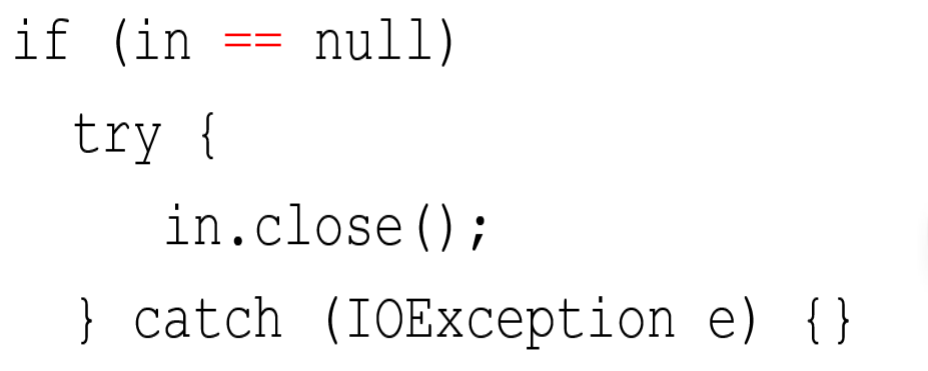
\includegraphics[width=0.50\textwidth]{figures/NullPointer1-1}
 \caption{Eclipse3.0.1中存在的空指针引用缺陷}\label{fig:figure1-1}
\end{figure}

\section{国内外研究现状及发展趋势}
%\label{sec:***} 可标注label

软件缺陷检测相关的研究几乎是伴随着软件的产生而出现的,随着程序设计语言的发展,软件缺陷类型也越来越多。通过人们对故障的总结,人们发现常见的比较大型的软件故障有数组越界,资源泄漏,空指针引用等,其中空指针引用问题出现的尤为频繁,根据coverity公司2009年针对280个开源项目的故障分析报告,空指针引用在所有类故障中所占比例为27.81\%,是所占比例最高的故障[11]。

以Java语言为例,Null关键字的广泛使用是Java代码中产生NPE(Null Pointer Exception)故障的直接原因,Haidar Osman\cite{osman2016tracking}等人开发了NullTracker工具对810个开源Java项目进行简单的数据流分析,追踪代码中空指针检查语句的分布情况,以发现程序开发者使用null关键字的时机和目的,结果表明在所有的条件判断语句中,用来进行空指针检查的语句平均占比为35\%,类成员没有初始化,方法返回null值,以及向方法中传递null值是引发NPE的最常见的因素。其中,71\%的空指针检查语句用来保证方法调用返回值的安全性。由于空指针检查语句的频繁使用,可能导致程序运行时的开销增加2\%-10\%,不仅如此,空指针检查的频繁使用还会降低代码的可读性和可维护性,而一旦缺失了这种检查,程序的稳定性便无法得到保障。

由于空指针引用故障在代码中广泛存在而又十分隐蔽,但是其一旦出现很大可能会导致程序崩溃,因此对程序的稳定性具有非常大的威胁。针对空指针引用缺陷的检测一直备受关注。

目前,代码缺陷检测的技术从大的层面上主要分为两大类,静态检测和动态检测。

动态检测\cite{wei2009safety}主要侧重于软件的性能、功能完善等方面,通过动态测试来进行漏洞的探测与发现,不仅仅要求测试人员对缺陷特性具有较深入的理解,测试过程中还需要大量测试用例,在目前软件规模愈加庞大,逻辑愈加复杂的情境下,这种方式必然带来大量的人力和物力的浪费。

静态检测\cite{lin2008static}是指利用静态分析手段来探测程序中潜在缺陷的方法,不需要运行程序使用其他手段完成对程序结构分析的技术。相较于动态分析技术而言,静态分析成本较低,而且能有效的对代码中的缺陷进行精确定位。因此,对源代码的静态分析和缺陷检测是一个值得深入研究的方向。


\section{本文研究内容}
%\label{sec:***} 可标注label
静态分析技术与工具具有较早发现缺陷、覆盖率高、低开销、自动化程序高等优点;同时静态分析技术也存在一定的局限性,不仅要在分析效率与精度中做出取舍,还需要在误报率与漏报率之间做出取舍。现有的一些静态检测工具(如Findbugs,PMD)都采用了不同的实现方法达到这样的平衡,由于采取的分析策略的不同,形成的检测结果也往往有较大差异。

基于当下Java代码空指针引用缺陷检测工具的特点,本文提出了利用交叉验证的方式整合不同工具的检测能力,以提高检测结果准确率的方法,同时利用深度学习方法,对复杂缺陷报告的判定构造决策模型。研究内容如下:

(1)首先基于SonarQube平台开发插件,集成多种静态代码分析工具对代码进行检测,然后把不同工具产生的检测报告进行交叉验证,将检测出的缺陷按照可信度优先级进行排序以提升检测报告的准确率。

(2)提出一种构建空指针引用缺陷测试用例的方法,并通过构造全局控制流图,抽取相应维度的代码特征的方式用含有结点特征的全局控制流图来描述测试用例。

(3)将含有特征信息控制流图转换成向量,利用深度学习的方法构建神经网络模型对多工具检测报告中矛盾缺陷的真实性进行评估,进一步优化BIT-Detector的检测结果。

\section{论文结构}
%\label{sec:***} 可标注label
第一章介绍了本文研究的背景,阐述了空指针引用缺陷检测的价值和意义,同时综述了国内外在空指针引用缺陷的静态检测方面研究的现状和发展趋势,最后表明了本文研究的主要内容。

第二章介绍了静态分析技术的特点和主要分析方法,并对比了这些方法的优点和不足之处,随后介绍了近年来静态分析方法在空指针引用缺陷检测的应用。本章还简要介绍了几种常用的静态代码分析工具,这些工具都可以用于Java代码的空指针引用缺陷检测。最后介绍了深度学习技术在软件安全领域的应用。

第三章是对本文工作进行总体的介绍,在设计背景部分,详细介绍了BIT-Detector设计的背景和试验效果并探讨了需要改进的地方,并引出后文深度学习模型的设计。然后介绍了BIT-Detector的工作环境和作业流程并详细阐述了利用深度模型提升检测效果的设计思路和工作流程。

第四章介绍了模型训练所需要的数据的来源和预处理过程。首先介绍了数据的来源和利用抽象语法树生成空指针引用缺陷的方法,然后依次介绍了测试用例控制流图的生成和利用过程间调用图生成全局控制流图的方式,随后还介绍了在代码特征提取阶段为了提取合适的代码特征怎样压缩全局控制流图。最后简单说明了数据的标注方式。

第五章分别介绍了图结构特征抽取模型和特征向量分类模型的构造方式,其中对深度学习涉及的一些基本概念进行了简单介绍,阐述了图数据特征抽取模型的理论基础以及设计原理,还介绍了分类模型神经网络的连接方式。最后阐明了神经网络的训练方法以及评判标准。 

第六章为实验部分,该部分首先介绍了实验的环境和数据的选取,然后对为不同工具设计的分类模型分别进行验证实验,最后使用相应数据集针对工具实际测试的结果和分类模型判定的结果进行综合实验,分析模型对于复杂检测报告缺陷真实性的鉴别能力。

最后总结部分对论文的工作进行总结和展望,探讨本文工作的价值和需要改进的地方。
